
\chapter{常に脚軌道生成が可能な自由歩容パターン生成手法を用いた実機実験}\label{chapter:常に脚軌道生成が可能な自由歩容パターン生成手法を用いた実機実験}

\chref{chapter:常に脚軌道生成が可能な自由歩容パターン生成手法を用いた実機実験}では,
実機を用いた歩行実験を行い,
本研究で提案した自由歩容パターン生成手法によって脚軌道生成の失敗が生じないことを示す.

\section{実験目的}
\chref{chapter:再評価手法の有効性の確認のための歩行シミュレーション}では,シミュレーションを用いて,
先行研究で歩行することができなかった地形で,脚軌道生成の失敗をすることなく歩行することができることを示した.
しかし,本研究で用いたシミュレーション環境では脚先の滑りによるずれやモータのトルクを考慮してない.
そのため,実機を用いた歩行実験を行い,
実際に本研究で提案した自由歩容パターン生成手法によって,
先行研究で歩行することができなかった地形で,
脚軌道生成の失敗をすることなく歩行することができることを確認することを目的とする.

本章では,先行研究で歩行することができなかった130mmの段差の上りおよび下りを行い,
脚軌道生成の失敗をすることなく歩行することができることを示す.

\section{実験方法}
\subsection{歩行する地形}
ロボットが歩行する地形を\figref{fig:walking-terrain}に示す.
地形の材質には,滑りにくさや加工のしやすさなどの理由から,
建築用断熱材であるスタイロフォームを用いた.
また,地形は\figref{fig:walking-terrain}のように,右側が左側に比べて130mm高くなっている.
上り動作の際には左側から右側に向かって歩行させ,下り動作の際には右側から左側に向かって歩行させた.

% fig:walking-terrain
\begin{figure}[tb]
  \centering
  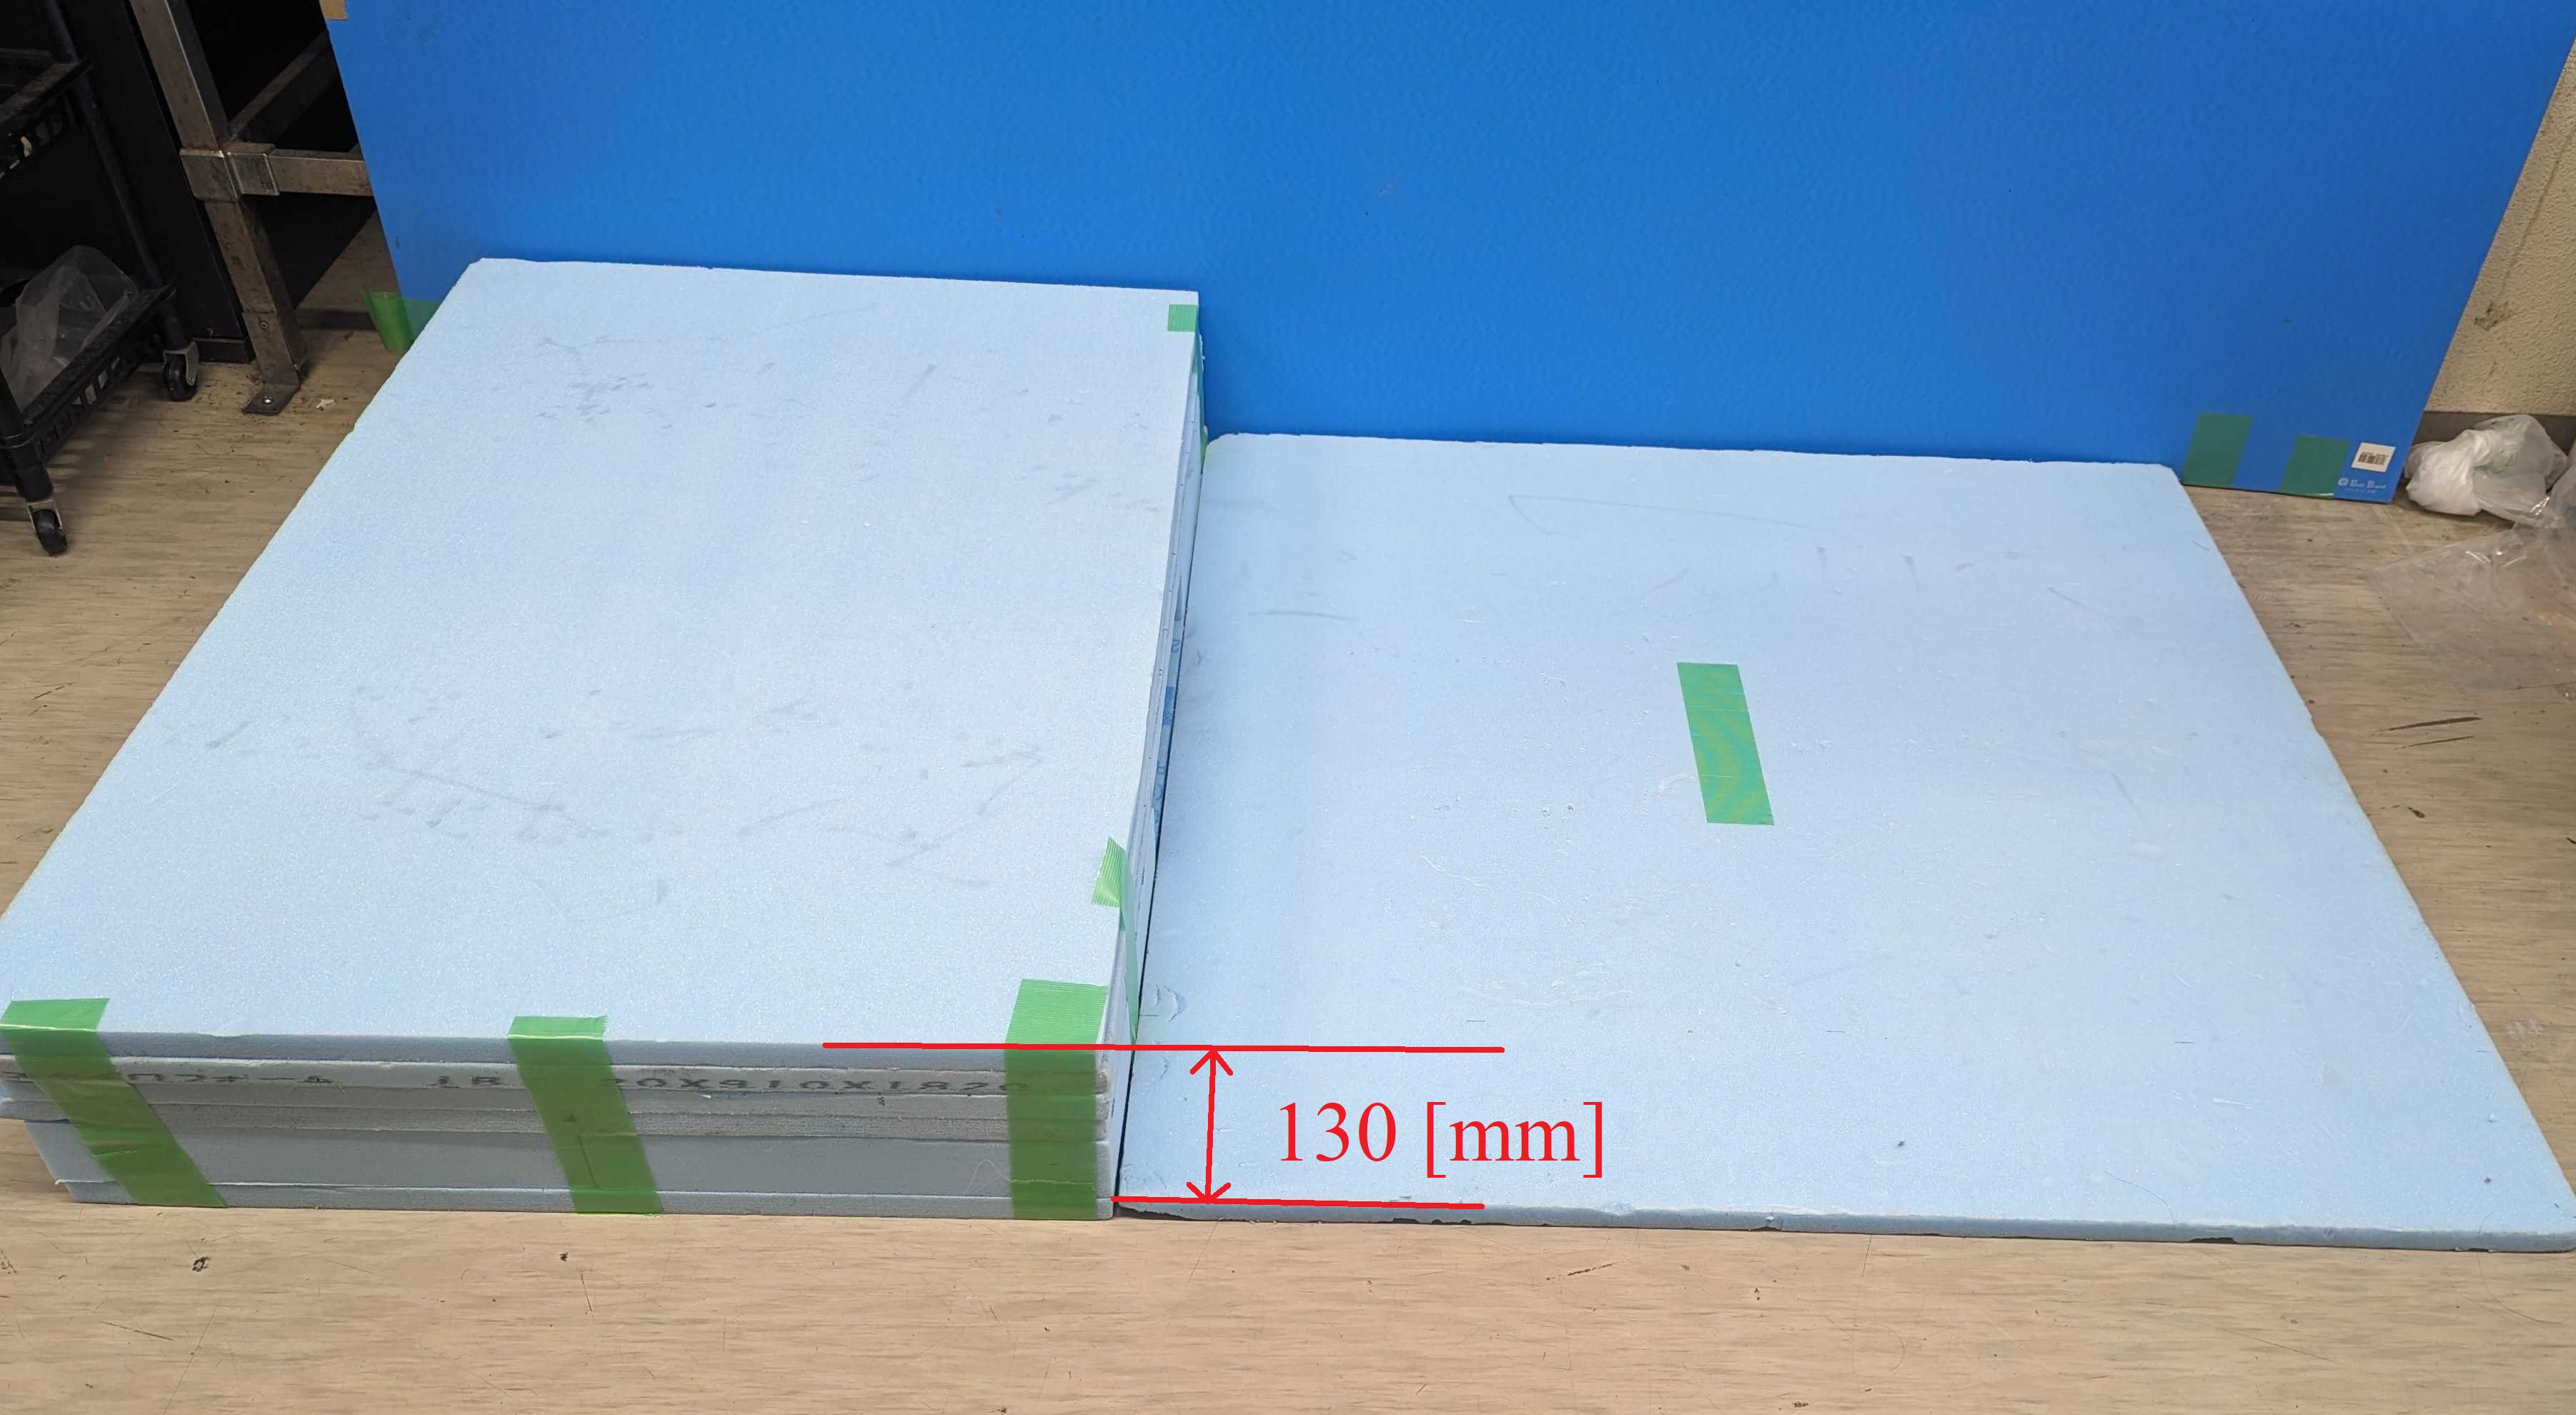
\includegraphics[width=0.8\linewidth]{figure/chapter5/walking-terrain.jpg}
  \caption{Walking Terrain}
  \label{fig:walking-terrain}
\end{figure}

\subsection{使用したロボット}
実験ではシミュレーションのモデルとしていたPhantomXを使用した.
内部電源では長時間稼働させるには容量が足りないため,
電源には外部電源として安定化電源($12V,5A$)を使用した.
ロボットへの指令値は,グラフ探索による自由歩容パターン生成手法を用いてPCで生成し,
XBeeを用いてPhantomXに送信した.

ロボットの脚軌道は矩形軌道を用いた.
また,本実験は先行研究では歩行ができなかった地形で歩行ができることを示すことが目的であるため,
地形は既知のものとし,地形の形状をセンサで計測することは行わなかった.

\subsection{歩行条件}
歩行実験時の歩行条件を以下に示す.

\begin{itemize}
  \item 胴体姿勢は常に地面と水平にする
  \item 動作は直進動作のみを行う
  \item ロボットの重心からみた遊脚高さは-20mmとする
  \item 安定余裕を15mmとする
  \item 胴体は地形から30mm以上離す
\end{itemize}

また,グラフ探索の条件を以下に示す.

\begin{itemize}
  \item 探索するグラフの深さは5とする
  \item 近似された可動範囲の最小半径は140mmとする
\end{itemize}

\section{結果}
実験の様子を以下に示す.


\section{考察}